%%%%%%%%%%%%%%%%%%%%%%%%%%%%%%%%%%%%%%%%%
% Classicthesis Typographic Thesis
% LaTeX Template
% Version 1.4 (1/1/16)
%
% This template has been downloaded from:
% http://www.LaTeXTemplates.com
%
% Original author:
% André Miede (http://www.miede.de) with commenting modifications by:
% Vel (vel@LaTeXTemplates.com)
%
% License:
% GNU General Public License (v2)
%
% General Tips:
% 1) Make sure to edit the classicthesis-config.file
% 2) New enumeration (A., B., C., etc in small caps): \begin{aenumerate} \end{aenumerate}
% 3) For margin notes: \marginpar or \graffito{}
% 4) Do not use bold fonts in this style, it is designed around them
% 5) Use tables as in the examples
% 6) See classicthesis-preamble.sty for useful commands
%
%%%%%%%%%%%%%%%%%%%%%%%%%%%%%%%%%%%%%%%%%

%----------------------------------------------------------------------------------------
%	PACKAGES AND OTHER DOCUMENT CONFIGURATIONS
%----------------------------------------------------------------------------------------

\documentclass[
		twoside,openright,titlepage,numbers=noenddot,headinclude,%1headlines,
	 	footinclude=true,cleardoublepage=empty,
		dottedtoc, % Make page numbers in the table of contents flushed right with dots leading to them
		BCOR=5mm,paper=a4,fontsize=11pt, % Binding correction, paper type and font size
		ngerman,american, % Languages, change this to your language(s)
		]{scrreprt} 
                
% Includes the file which contains all the document configurations and packages - make sure to edit this file
%%%%%%%%%%%%%%%%%%%%%%%%%%%%%%%%%%%%%%%%%
% Classicthesis Typographic Thesis
% Configuration File
%
% This file has been downloaded from:
% http://www.LaTeXTemplates.com
%
% Original author:
% André Miede (http://www.miede.de) with extensive commenting changes by:
% Vel (vel@LaTeXTemplates.com)
%
% License:
% GNU General Public License (v2)
%
% Important note:
% The main lines to change in this file are in the DOCUMENT VARIABLES
% section, the rest of the file is for advanced configuration.
%
%%%%%%%%%%%%%%%%%%%%%%%%%%%%%%%%%%%%%%%%%

%----------------------------------------------------------------------------------------
%	CHARACTER ENCODING
%----------------------------------------------------------------------------------------

\PassOptionsToPackage{utf8}{inputenc} % Set the encoding of your files. UTF-8 is the only sensible encoding nowadays. If you can't read äöüßáéçèê∂åëæƒÏ€ then change the encoding setting in your editor, not the line below. If your editor does not support utf8 use another editor!
\usepackage{inputenc}

%----------------------------------------------------------------------------------------
%	DOCUMENT VARIABLES
%	Fill in the lines below to enter your information into the thesis template
%	Each of the commands can be cited anywhere in the thesis
%----------------------------------------------------------------------------------------

% Remove drafting to get rid of the '[ Date - classicthesis version 4.0 ]' text at the bottom of every page
\PassOptionsToPackage{eulerchapternumbers,listings,drafting, pdfspacing, subfig,beramono,eulermath,parts}{classicthesis}
% Available options: drafting parts nochapters linedheaders eulerchapternumbers beramono eulermath pdfspacing minionprospacing tocaligned dottedtoc manychapters listings floatperchapter subfig

\newcommand{\myTitle}{A Classic Thesis Style\xspace}
\newcommand{\mySubtitle}{An Homage to The Elements of Typographic Style\xspace}
\newcommand{\myDegree}{Bachelor of Information Technology (Honours)\xspace}
\newcommand{\myName}{Yiping Su\xspace}
% \newcommand{\myProf}{Cheng Soon Ong \xspace}
\newcommand{\myOtherProf}{Put name here\xspace}
\newcommand{\mySupervisor}{Cheng Soon Ong\xspace}
\newcommand{\myFaculty}{Put data here\xspace}
\newcommand{\myDepartment}{College of Engineering and Computer Science\xspace}
\newcommand{\myUni}{Australian National University\xspace}
\newcommand{\myLocation}{Canberra\xspace}
\newcommand{\myTime}{June 2020\xspace}
\newcommand{\myVersion}{version 0.7\xspace}

%----------------------------------------------------------------------------------------
%	USEFUL COMMANDS
%----------------------------------------------------------------------------------------

\newcommand{\ie}{i.\,e.}
\newcommand{\Ie}{I.\,e.}
\newcommand{\eg}{e.\,g.}
\newcommand{\Eg}{E.\,g.} 

\newcounter{dummy} % Necessary for correct hyperlinks (to index, bib, etc.)
\providecommand{\mLyX}{L\kern-.1667em\lower.25em\hbox{Y}\kern-.125emX\@}
\newlength{\abcd} % for ab..z string length calculation

%----------------------------------------------------------------------------------------
%	PACKAGES
%----------------------------------------------------------------------------------------

\usepackage{lipsum} % Used for inserting dummy 'Lorem ipsum' text into the template

%------------------------------------------------

%\PassOptionsToPackage{ngerman,american}{babel}  % Change this to your language(s)
% Spanish languages need extra options in order to work with this template
%\PassOptionsToPackage{spanish,es-lcroman}{babel}
\usepackage{babel}

%------------------------------------------------			

\usepackage{csquotes}
\PassOptionsToPackage{%
% backend=biber, % Instead of bibtex
backend=bibtex8,bibencoding=ascii,%
language=auto,%
style=numeric-comp,%
%style=authoryear-comp, % Author 1999, 2010
%bibstyle=authoryear,dashed=false, % dashed: substitute rep. author with ---
sorting=nyt, % name, year, title
maxbibnames=10, % default: 3, et al.
%backref=true,%
natbib=true % natbib compatibility mode (\citep and \citet still work)
}{biblatex}
\usepackage{biblatex}
 
 %------------------------------------------------

\PassOptionsToPackage{fleqn}{amsmath} % Math environments and more by the AMS 
 \usepackage{amsmath}

 %------------------------------------------------

\PassOptionsToPackage{T1}{fontenc} % T2A for cyrillics
\usepackage{fontenc}

%------------------------------------------------

\usepackage{textcomp} % Fix warning with missing font shapes

%------------------------------------------------

\usepackage{scrhack} % Fix warnings when using KOMA with listings package  

%------------------------------------------------

\usepackage{xspace} % To get the spacing after macros right

%------------------------------------------------

\usepackage{mparhack} % To get marginpar right

%------------------------------------------------

\usepackage{fixltx2e} % Fixes some LaTeX stuff 

%------------------------------------------------

\PassOptionsToPackage{smaller}{acronym} % Include printonlyused in the first bracket to only show acronyms used in the text
\usepackage{acronym} % Nice macros for handling all acronyms in the thesis

%\renewcommand*{\acsfont}[1]{\textssc{#1}} % For MinionPro
\renewcommand*{\aclabelfont}[1]{\acsfont{#1}}

%------------------------------------------------

\PassOptionsToPackage{pdftex}{graphicx}
\usepackage{graphicx} 

%----------------------------------------------------------------------------------------
%	FLOATS: TABLES, FIGURES AND CAPTIONS SETUP
%----------------------------------------------------------------------------------------

\usepackage{tabularx} % Better tables
\setlength{\extrarowheight}{3pt} % Increase table row height
\newcommand{\tableheadline}[1]{\multicolumn{1}{c}{\spacedlowsmallcaps{#1}}}
\newcommand{\myfloatalign}{\centering} % To be used with each float for alignment
\usepackage{caption}
\captionsetup{font=small}
\usepackage{subfig}  

%----------------------------------------------------------------------------------------
%	CODE LISTINGS SETUP
%----------------------------------------------------------------------------------------

\usepackage{listings} 
%\lstset{emph={trueIndex,root},emphstyle=\color{BlueViolet}}%\underbar} % For special keywords
\lstset{language=[LaTeX]Tex,%C++ % Specify the language(s) for listings here
morekeywords={PassOptionsToPackage,selectlanguage},
keywordstyle=\color{RoyalBlue}, % Add \bfseries for bold
basicstyle=\small\ttfamily, % Makes listings a smaller font size and a different font
%identifierstyle=\color{NavyBlue}, % Color of text inside brackets
commentstyle=\color{Green}\ttfamily, % Color of comments
stringstyle=\rmfamily, % Font type to use for strings
numbers=left, % Change left to none to remove line numbers
numberstyle=\scriptsize, % Font size of the line numbers
stepnumber=5, % Increment of line numbers
numbersep=8pt, % Distance of line numbers from code listing
showstringspaces=false, % Sets whether spaces in strings should appear underlined
breaklines=true, % Force the code to stay in the confines of the listing box
%frameround=ftff, % Uncomment for rounded frame
%frame=single, % Frame border - none/leftline/topline/bottomline/lines/single/shadowbox/L
belowcaptionskip=.75\baselineskip % Space after the "Listing #: Desciption" text and the listing box
}

%----------------------------------------------------------------------------------------
%	HYPERREFERENCES
%----------------------------------------------------------------------------------------

\PassOptionsToPackage{pdftex,hyperfootnotes=false,pdfpagelabels}{hyperref}
\usepackage{hyperref}  % backref linktocpage pagebackref
\pdfcompresslevel=9
\pdfadjustspacing=1

\hypersetup{
% Uncomment the line below to remove all links (to references, figures, tables, etc), useful for b/w printouts
%draft, 
colorlinks=true, linktocpage=true, pdfstartpage=3, pdfstartview=FitV,
% Uncomment the line below if you want to have black links (e.g. for printing black and white)
%colorlinks=false, linktocpage=false, pdfborder={0 0 0}, pdfstartpage=3, pdfstartview=FitV, 
breaklinks=true, pdfpagemode=UseNone, pageanchor=true, pdfpagemode=UseOutlines,%
plainpages=false, bookmarksnumbered, bookmarksopen=true, bookmarksopenlevel=1,%
hypertexnames=true, pdfhighlight=/O,%nesting=true,%frenchlinks,%
urlcolor=webbrown, linkcolor=RoyalBlue, citecolor=webgreen, %pagecolor=RoyalBlue,%
    %urlcolor=Black, linkcolor=Black, citecolor=Black, %pagecolor=Black,%
%------------------------------------------------
% PDF file meta-information
pdftitle={\myTitle},
pdfauthor={\textcopyright\ \myName, \myUni, \myFaculty},
pdfsubject={},
pdfkeywords={},
pdfcreator={pdfLaTeX},
pdfproducer={LaTeX with hyperref and classicthesis}
%------------------------------------------------
}

%----------------------------------------------------------------------------------------
%	AUTOREFERENCES SETUP
%	Redefines how references in text are prefaced for different 
%	languages (e.g. "Section 1.2" or "section 1.2")
%----------------------------------------------------------------------------------------

\makeatletter
\@ifpackageloaded{babel}
{
\addto\extrasamerican{
\renewcommand*{\figureautorefname}{Figure}
\renewcommand*{\tableautorefname}{Table}
\renewcommand*{\partautorefname}{Part}
\renewcommand*{\chapterautorefname}{Chapter}
\renewcommand*{\sectionautorefname}{Section}
\renewcommand*{\subsectionautorefname}{Section}
\renewcommand*{\subsubsectionautorefname}{Section}
}
\addto\extrasngerman{
\renewcommand*{\paragraphautorefname}{Absatz}
\renewcommand*{\subparagraphautorefname}{Unterabsatz}
\renewcommand*{\footnoteautorefname}{Fu\"snote}
\renewcommand*{\FancyVerbLineautorefname}{Zeile}
\renewcommand*{\theoremautorefname}{Theorem}
\renewcommand*{\appendixautorefname}{Anhang}
\renewcommand*{\equationautorefname}{Gleichung}
\renewcommand*{\itemautorefname}{Punkt}
}
\providecommand{\subfigureautorefname}{\figureautorefname} % Fix to getting autorefs for subfigures right
}{\relax}
\makeatother

%----------------------------------------------------------------------------------------

\usepackage{classicthesis} 

%----------------------------------------------------------------------------------------
%	CHANGING TEXT AREA 
%----------------------------------------------------------------------------------------

%\linespread{1.05} % a bit more for Palatino
% \areaset[current]{400pt}{761pt} % 686 (factor 2.2) + 33 head + 42 head \the\footskip
\setlength{\marginparwidth}{9em}%
% \setlength{\marginparsep}{2em}%

%----------------------------------------------------------------------------------------
%	USING DIFFERENT FONTS
%----------------------------------------------------------------------------------------

%\usepackage[oldstylenums]{kpfonts} % oldstyle notextcomp
%\usepackage[osf]{libertine}
%\usepackage[light,condensed,math]{iwona}
%\renewcommand{\sfdefault}{iwona}
%\usepackage{lmodern} % <-- no osf support :-(
%\usepackage{cfr-lm} % 
%\usepackage[urw-garamond]{mathdesign} <-- no osf support :-(
%\usepackage[default,osfigures]{opensans} % scale=0.95 
%\usepackage[sfdefault]{FiraSans}


% \usepackage[margin=1in]{geometry}
\usepackage{amssymb}
% \usepackage{amsmath}
\usepackage{bm}
% \usepackage{xcolor}

% \usepackage[english]{babel}
% \usepackage[utf8]{inputenc}
\usepackage{algorithm}
% \usepackage{algpseudocode}
% \usepackage{algorithmic}
\usepackage[noend]{algpseudocode}
\usepackage{enumitem}

\usepackage{float}
% \usepackage{graphicx} % Required for inserting images
% \usepackage{subcaption}

\graphicspath{{Figures/}{./}} 

\def\R{\mathrm I\!R}
\def\x{\bm{x}}
\DeclareMathOperator*{\argmax}{arg\,max}
\DeclareMathOperator*{\argmin}{arg\,min}

\renewcommand{\algorithmicrequire}{\textbf{Input:}}
\renewcommand{\algorithmicensure}{\textbf{Output:}}

\addbibresource{Bibliography.bib} % The file housing your bibliography
%\addbibresource[label=ownpubs]{Self_Publications.bib} % Uncomment for optional self-publications

%\hyphenation{Put special hyphenation here}

\begin{document}

\frenchspacing % Reduces space after periods to make text more compact

\raggedbottom % Makes all pages the height of the text on that page

\selectlanguage{american} % Select your default language - e.g. american or ngerman

%\renewcommand*{\bibname}{new name} % Uncomment to change the name of the bibliography
%\setbibpreamble{} % Uncomment to include a preamble to the bibliography - some text before the reference list starts

\pagenumbering{roman} % Roman page numbering prior to the start of the thesis content (i, ii, iii, etc)

\pagestyle{plain} % Suppress headers for the pre-content pages

%----------------------------------------------------------------------------------------
%	PRE-CONTENT THESIS PAGES
%----------------------------------------------------------------------------------------

% % Title Page

\begin{titlepage}

\begin{addmargin}[-1cm]{-3cm}
\begin{center}
\large

\hfill
\vfill

\begingroup
\color{Maroon}\spacedallcaps{Quantile estimation on streaming data} \\ \bigskip % Thesis title
\endgroup

\spacedlowsmallcaps{Yiping Su} % Your name

\vfill


\includegraphics[width=6cm]{Figures/ANU_Logo} \\ \bigskip % Picture

A study on something I don't quite understand yet \\ \bigskip \bigskip % Thesis subtitle
\myDegree \\
\myDepartment \\
%\myFaculty \\
\myUni \\ 
\bigskip \bigskip

February 2020 -- \myVersion % Time and version

\vfill

\end{center}
\end{addmargin}

\end{titlepage} % Main title page

% % Back of the title page

\thispagestyle{empty}

\hfill

\vfill

\noindent\myName: \textit{\myTitle,} \mySubtitle, %\myDegree, 
\textcopyright\ \myTime

% You may wish to do something with the back of the title page, such as including your supervisors, location or time frame of the work. Below is an example of doing so although you may want to tweak it to your liking.

%\bigskip

%\noindent\spacedlowsmallcaps{Supervisors}: \\
%\myProf \\
%\myOtherProf \\ 
%\mySupervisor

%\medskip \\

%\noindent\spacedlowsmallcaps{Location}: \\
%\myLocation

%\medskip \\

%\noindent\spacedlowsmallcaps{Time Frame}: \\
%\myTime
 % Back of the title page

% \cleardoublepage% Dedication

\thispagestyle{empty}
\refstepcounter{dummy}

\pdfbookmark[1]{Dedication}{Dedication} % Bookmark name visible in a PDF viewer

\vspace*{3cm}

\begin{center}
\emph{Ohana} means family. \\
Family means nobody gets left behind, or forgotten. \\ \medskip
--- Lilo \& Stitch    
\end{center}

\medskip

\begin{center}
Dedicated to the loving memory of Rudolf Miede. \\ \smallskip
1939\,--\,2005
\end{center} % Dedication page

%\cleardoublepage\include{FrontBackMatter/Foreword} % Uncomment and create a Foreword.tex to include a foreword

% \cleardoublepage% Abstract

%\renewcommand{\abstractname}{Abstract} % Uncomment to change the name of the abstract

\pdfbookmark[1]{Abstract}{Abstract} % Bookmark name visible in a PDF viewer

\begingroup
\let\clearpage\relax
\let\cleardoublepage\relax
\let\cleardoublepage\relax

\chapter*{Abstract}
Short summary of the contents\dots a great guide by 
Kent Beck how to write good abstracts can be found here:  
\begin{center}
\url{https://plg.uwaterloo.ca/~migod/research/beckOOPSLA.html}
\end{center}

\endgroup			

\vfill % Abstract page

% \cleardoublepage% Publications - a page listing research articles written using content in the thesis

\pdfbookmark[1]{Publications}{Publications} % Bookmark name visible in a PDF viewer

\chapter*{Publications} % Publications page text

Some ideas and figures have appeared previously in the following publications:\\

\noindent Put your publications from the thesis here. The packages \texttt{multibib} or \texttt{bibtopic} etc. can be used to handle multiple different bibliographies in your document.

%\begin{refsection}[ownpubs]
%    \small
%    \nocite{*} % is local to to the enclosing refsection
%    \printbibliography[heading=none]
%\end{refsection}

%\emph{Attention}: This requires a separate run of \texttt{bibtex} for your \texttt{refsection}, \eg, \texttt{ClassicThesis1-blx} for this file. You might also use \texttt{biber} as the backend for \texttt{biblatex}. See also \url{http://tex.stackexchange.com/questions/128196/problem-with-refsection}. % Publications from the thesis page

% \cleardoublepage% Acknowledgements

\pdfbookmark[1]{Acknowledgements}{Acknowledgements} % Bookmark name visible in a PDF viewer

\begin{flushright}{\slshape    
We have seen that computer programming is an art, \\ 
because it applies accumulated knowledge to the world, \\ 
because it requires skill and ingenuity, and especially \\
because it produces objects of beauty.} \\ \medskip
--- \defcitealias{knuth:1974}{Donald E. Knuth}\citetalias{knuth:1974} \citep{knuth:1974}
\end{flushright}

\bigskip

%----------------------------------------------------------------------------------------

\begingroup

\let\clearpage\relax
\let\cleardoublepage\relax
\let\cleardoublepage\relax

\chapter*{Acknowledgements}

\noindent Put your acknowledgements here.\\

\noindent Many thanks to everybody who already sent me a postcard!\\

\noindent Regarding the typography and other help, many thanks go to Marco Kuhlmann, Philipp Lehman, Lothar Schlesier, Jim Young, Lorenzo Pantieri and Enrico Gregorio\footnote{Members of GuIT (Gruppo Italiano Utilizzatori di \TeX\ e \LaTeX )}, J\"org Sommer, Joachim K\"ostler, Daniel Gottschlag, Denis Aydin, Paride Legovini, Steffen Prochnow, Nicolas Repp, Hinrich Harms, Roland Winkler, and the whole \LaTeX-community for support, ideas and some great software.

\bigskip

\noindent\emph{Regarding \mLyX}: The \mLyX\ port was initially done by
\emph{Nicholas Mariette} in March 2009 and continued by
\emph{Ivo Pletikosi\'c} in 2011. Thank you very much for your work and the contributions to the original style.

\endgroup % Acknowledgements page

\pagestyle{scrheadings} % Show chapter titles as headings

% \cleardoublepage% Table of Contents - List of Tables/Figures/Listings and Acronyms

\refstepcounter{dummy}

\pdfbookmark[1]{\contentsname}{tableofcontents} % Bookmark name visible in a PDF viewer

\setcounter{tocdepth}{2} % Depth of sections to include in the table of contents - currently up to subsections

\setcounter{secnumdepth}{3} % Depth of sections to number in the text itself - currently up to subsubsections

\manualmark
\markboth{\spacedlowsmallcaps{\contentsname}}{\spacedlowsmallcaps{\contentsname}}
\tableofcontents 
\automark[section]{chapter}
\renewcommand{\chaptermark}[1]{\markboth{\spacedlowsmallcaps{#1}}{\spacedlowsmallcaps{#1}}}
\renewcommand{\sectionmark}[1]{\markright{\thesection\enspace\spacedlowsmallcaps{#1}}}

\clearpage

\begingroup 
\let\clearpage\relax
\let\cleardoublepage\relax
\let\cleardoublepage\relax

%----------------------------------------------------------------------------------------
%	List of Figures
%----------------------------------------------------------------------------------------
    
% \refstepcounter{dummy}
% %\addcontentsline{toc}{chapter}{\listfigurename} % Uncomment if you would like the list of figures to appear in the table of contents
% \pdfbookmark[1]{\listfigurename}{lof} % Bookmark name visible in a PDF viewer

% \listoffigures

% \vspace{8ex}
% \newpage

%----------------------------------------------------------------------------------------
%	List of Tables
%----------------------------------------------------------------------------------------

% \refstepcounter{dummy}
% %\addcontentsline{toc}{chapter}{\listtablename} % Uncomment if you would like the list of tables to appear in the table of contents
% \pdfbookmark[1]{\listtablename}{lot} % Bookmark name visible in a PDF viewer

% \listoftables
        
% \vspace{8ex}
% \newpage
    
%----------------------------------------------------------------------------------------
%	List of Listings
%---------------------------------------------------------------------------------------- 

% \refstepcounter{dummy}
% %\addcontentsline{toc}{chapter}{\lstlistlistingname} % Uncomment if you would like the list of listings to appear in the table of contents
% \pdfbookmark[1]{\lstlistlistingname}{lol} % Bookmark name visible in a PDF viewer

% \lstlistoflistings 

% \vspace{8ex}
% \newpage
       
%----------------------------------------------------------------------------------------
%	Acronyms
%----------------------------------------------------------------------------------------

% \refstepcounter{dummy}
% %\addcontentsline{toc}{chapter}{Acronyms} % Uncomment if you would like the acronyms to appear in the table of contents
% \pdfbookmark[1]{Acronyms}{acronyms} % Bookmark name visible in a PDF viewer

% \markboth{\spacedlowsmallcaps{Acronyms}}{\spacedlowsmallcaps{Acronyms}}

% \chapter*{Acronyms}

% \begin{acronym}[UML]
% \acro{DRY}{Don't Repeat Yourself}
% \acro{API}{Application Programming Interface}
% \acro{UML}{Unified Modeling Language}
% \end{acronym}  
                   
\endgroup

 % Contents, list of figures/tables/listings and acronyms

% \cleardoublepage

\pagenumbering{arabic} % Arabic page numbering for thesis content (1, 2, 3, etc)
%\setcounter{page}{90} % Uncomment to manually start the page counter at an arbitrary value (for example if you wish to count the pre-content pages in the page count)

% \cleardoublepage % Avoids problems with pdfbookmark



% \ctparttext{You can put some informational part preamble text here. Illo principalmente su nos. Non message \emph{occidental} angloromanic da. Debitas effortio simplificate sia se, auxiliar summarios da que, se avantiate publicationes via. Pan in terra summarios, capital interlingua se que. Al via multo esser specimen, campo responder que da. Le usate medical addresses pro, europa origine sanctificate nos se.} % Text on the Part 1 page describing  the content in Part 1

% \part{Some Kind of Manual} % First part of the thesis

%----------------------------------------------------------------------------------------
%	THESIS CONTENT - CHAPTERS
%----------------------------------------------------------------------------------------

% \documentclass[12pt]{article}
\usepackage{xcolor}
\def\R{\rm I\!R}
\def\x{\bm{x}}
\usepackage[numbers]{natbib}

\title{Literature review outline}
\date{\vspace{-5ex}}


\begin{document}
\maketitle

\section{SGD 
            \color{blue}{(should it be in Background instead?)}}
    

\section{Quantile Estimation From Streaming Data}
\begin{enumerate}
    \item Why useful: \\
        \cite{rayArtApproximatingDistributions1800}(Industrial use) "
        Many businesses care about accurately computing quantiles over their key metrics, which can pose several interesting challenges at scale. 

        e.g. Price for advertisement on bidding level: quantile estimation helps price setting
        "\\\\
        Other industrial usage mentioned in \cite{hongEstimatingQuantileSensitivities2009}, and its citations for industrial use \\
        "
        Quantiles have been adopted by many industries as major
        measures of random performance. In the financial industry,
        quantiles, also known as value-at-risks (VaRs), are widely
        accepted measures of capital adequacy. For example, the
        Bank for International Settlement uses the 10-day VaR at
        the 99\% level to measure the adequacy of bank capital
        (Duffie and Pan 1997). In the service industry, quantiles
        are often used as measures of service quality. For example, the service quality of an out-of-hospital system is frequently measured by the 90th percentile of the times taken
        to respond to emergency requests and to transport patients
        to a hospital (Austin and Schull 2003). Quantiles have
        also been used as billing measures in some circumstances.
        For example, some Internet service providers (ISPs) charge
        their users based on the 95th percentile of the traffic load
        in a billing cycle (Goldenberg et al. 2004).
        "
    % \item Pinball loss on quantile regression: \\
    %     \cite{steinwartEstimatingConditionalQuantiles2011}\\
    %     \cite{koenkerRegressionQuantiles1978}
    % \item Simultaneously predicting several quantiles: \\
    %     \cite{sangnierJointQuantileRegression} (non-streaming)(multi-dimensional)(quantile regression)\\
    \item Quantile Streaming: \\
        \cite{greenwaldQuantilesEquidepthHistograms2016}\\
        They propose a property on quantile estimation which guarantees accuracy within a pre-specified precision. 
        \textbf{$\epsilon$-approximate $\phi$-quantile}
        It is good(????) for algorithms with equidepth histogram method.
        A new algorithm for $\epsilon$-approximate quantiles with space complexity $O(log(\epsilon n)/\epsilon)$ is proposed. It is inspired by \textbf{Manku, Rajagopalan}'s work. 
         The problem is, the memory passes into the device(???) is affected by data size.
        \\\\
        \cite{maFrugalStreamingEstimating2014}\\
    \pagebreak    
    \item Parallel estimation \textbf{on other things} from Streaming Data: \\
        % \cite{jainP2AlgorithmDynamic1985}\\
        Related work on parallel quantile estimation on streaming data.



        Multiple quantile estimation from streaming data requires the estimation of several different quantile values being calculated simultaneously from streaming data. It has been an issue targeted by different algorithms.\\\\

        \cite{ben-haimStreamingParallelDecision} 
        \textbf{A Streaming Parallel Decision Tree Algorithm}

        The Streaming Parallel Decision Tree (SPDT) algorithm \cite{ben-haimStreamingParallelDecision} introduces an on-line histogram building method % from streaming data at parallel processors.
        in which histogram boundaries are estimated quantile values.
        In this method, multiple histograms are built from streaming data in parallel, which are then merged into a summary histogram of the entire dataset. The summary histogram is a set of sorted real numbers that represents the interval boundaries such that all the intervals have approximately the same size. Specifically, for a summary histogram with $N$ intervals, the set of real numbers is approximately the set of $\tau$-quantiles ($\tau = \frac{1}{N}, \frac{2}{N}, ..., \frac{N-1}{N}$) for the input data stream.

        This method works for distributed system where big data stream is processed by different processors. It also works well for huge amount of data because the computation complexity is not affected by the size of dataset.
        % This summary histogram is notable for its evenly distributed intervals sizes, as each interval has the same number of data points. To interpret the histogram into quantiles, 
        \\\\
        \cite{pebayFormulasRobustOnepass2008}\\

\end{enumerate}

\section{Anomaly Detection and Outlier}

\begin{enumerate}
    \item Anomaly detection: \\
        \cite{emmottMetaAnalysisAnomalyDetection2015}
        (industrial use)
        ()
        % \cite{huangOnlineAnomalousTime2013}
\end{enumerate}
\newpage
\textbf{My work} Quantile estimation on streaming data, which would be applied on 

\newpage
% \citeauthor{blassWhenAreTwo2008}
\bibliography{Thesis}
\bibliographystyle{IEEEtranN}

\end{document}
\end(documentclass) % Chapter 1
% \chapter{Stochastic Average Gradient}
\label{ch: SAG}

\section{Introduction}
The stochastic average gradient (SAG)\cite{schmidtMinimizingFiniteSums2016} is an convex optimization method that has a significant improvement of convergence rate than stochastic gradient (SG) methods. In general, the convergence rate is improved from $O(1/\sqrt{k})$ to $O(1/k)$, reaching the same level as the gradient descent method. Along with the rising convergence rate, it keeps a low computational cost for each iteration to be independent from the size of function sum.

\subsection{Machenism of SAG}
Similar to SG methods, SAG methods aim for minimization of the sum of a finite number of smooth convex functions where $n$ is very large. The problem setting is
$$
\underset{x \in \mathbb{R}^p}{\text{minimize}} g(x) := \frac{1}{n}\sum^n_{i=1} f_i(x)
$$
where each $f_i$ is a smooth convex function.

The standard (full) gradient (FG) method has each iteration in the form
$$
x_{k+1} = x_k - \alpha_k g\prime (x_k) = x_k - \frac{\alpha_k}{n}\sum^n_{i=1} f_i\prime(x_k)
$$
where $\alpha_k$ is the step size of iteration $k$. For each iteration, the computational cost is $O(n)$.

To save the iteration cost, the stochastic gradient (SG) method has each iteration in the form
$$
x_{k+1} = x_k - \alpha_k f_{i_k}\prime (x_k)
$$
where $i_k$ is the index for the iteration that gets sampled from the range {$1, 2,...,n$}. It has an iteration cost of $O(1)$, but a much lower convergence rate.

The stochastic average gradient (SAG) remembers the last update of a gradient value for each index $i$, which enables the improvement of convergence rate from SG methods. Its iteration takes the form
$$
x_{k+1} = x_k - \frac{\alpha_k}{n} \sum^n_{i=1}y_{i}^{k}
$$
where $y_{i}^{k}$ is used to keep the memory of recently updated gradient value of function $f_i$
$$
y_{i}^{k}:=\left\{\begin{array}{ll}
    f_{i}^{\prime}\left(x_{k}\right) & \text { if } i=i_{k} \\
    y_{i}^{k-1} & \text { otherwise }
    \end{array}\right.
$$
The SAG algorithm, according to \citeauthor{schmidtMinimizingFiniteSums2016}, "like the FG method, the step incorporates a gradient with respect to each function". Meanwhile only one gradient computation is involved in the combination of gradients, such that the iteration cost is independent of $n$.

\subsection{Convergence guarantee}

Under the assumption that each $f_i$ is convex and the gradient $f_i\prime$ is \textit{Lipschitz continuous} with constant $L$, which means
$$
|f_i\prime (a) - f_i\prime (b)| \leq L|a-b|
$$
for all $a,b \in \mathbb{R}^p$.
The SAG algorithm with constant step size $\alpha_k = \frac{1}{16L}$ reaches the convergence rate of $O(1/k)$. The convergence function differs when the $y_i^0$ is initialized differently, or when $f_i$ is strongly convex.


\section{Basic SAG algorithm}

\begin{algorithm}
    \caption{Basic SAG method for minimizing $\frac{1}{n} \sum^n_{i=1}f_i(x)$ with step size $\alpha$}\label{alg:SAG_ori}
        \begin{algorithmic}[1]
            \Require{Dataset $X$, Dataset Size $n$, Step size $\alpha$}
            \Ensure{$x$}
            % \Procedure{frugal}{$X,\tau$}            \Comment{X is the dataset}
            \State {$d = 0, y_i = 0$ for $i = 1, 2, ..., n$}           \Comment{Default initialization}
            \For{$k = 0,1,...$ \textbf{do}}                  %\Comment{Parameter update for each input data point}
                \State {Sample $i$ from {$1,2,...,n$}}
                \State {$d=d - y_i + f^{\prime}_i(x))$}
                \State {$y_i = f^{\prime}_i(x)$}
                \State{$x = x - \frac{\alpha}{n}d$}
            \EndFor
            \State{\textbf{end for}}
        \end{algorithmic}
\end{algorithm}

The Basic SAG algorithm requires memory storage of a table of $y_i (i= 1, 2, ...,n)$, to keep the track of each $y_i$ in case they are re-visited after first update.

\section{Basic SAG Implementation on quantile estimation}

The quantile estimation loss function is a convex function, and \textbf{we can use a smooth function for replacement}
\begin{algorithm}
    \caption{Basic SAG method for streaming data $S$ for quantile estimation}\label{alg:SAG}
        \begin{algorithmic}[1]
            \Require{Data Stream $S$, Data Stream Size $n$, $\tau$, $\tau$-quantile estimate $\tilde{q}$, Step size $\alpha$}
            \Ensure{$\tilde{q}$}
            % \Procedure{frugal}{$X,\tau$}            \Comment{X is the dataset}
            \State {Initialization $d = 0, \tilde{q}=0$}           \Comment{Default initialization $q_0=0$, $d_0=0$}
            \For{\textbf{each} $s_i$ in $S$}                  %\Comment{Parameter update for each input data point}
                \State {$d=d - 0 + l^{\prime}_{\tau}(s_i, \tilde{q})$} \Comment{$0$ stands for $y_i^{k-1}$}
                % \State {\textbf{set} $\alpha_k$} \Comment{Set stepsize}
                \State{$\tilde{q} = \tilde{q} - \frac{\alpha}{n}d$}
            \EndFor
            \State{\textbf{end for}}
        \end{algorithmic}
\end{algorithm}
For streaming data, it's worthwhile noticing that each input data point has one and only one pass. Which means for the SAG implementation, the storage of updated $y_i^k$ is useless since it would not be revisited. Besides, if all $y_i^0$ are initialized as 0, the storage of $y^0$ initialization needs only one unit of memory instead of $n$ units of memory. in this way, we can keep the memory complexity of SAG quantile estimation to $O(1)$.



\chapter{Smooth Functions}
\label{ch: smooth_func}

\graphicspath{{Figures/Smooth_func/}{./}} 
\textbf{This is a section not a chapter}


\section{Smooth Functions}
The pinball loss function we use for the SGD quantile estimation is convex but not smooth. 
Theoretically, however, both SGD and SAG methods need smoothness for the guarantee of convergence. Although the practical experiments have shown that there is evidence of convergence in final performance, it remains a serious problem for our SGD quantile estimation methods. In this section, we present the analysis on the non-smoothness problem, followed by the potential solutions and further discussions on them.

\subsection{The Pinball Loss Functions}
The pinball loss function evaluates the loss from a data point $x$ for estimation of the $\tau$-quantile.

\textbf{quote the equation of pinball loss function and it's derivative}

The fact that the pinball loss function is not differentiable at $x= 0$ has became a problem for the stochastic gradient descent which uses derivatives of object functions.

\begin{figure*}[h!]
	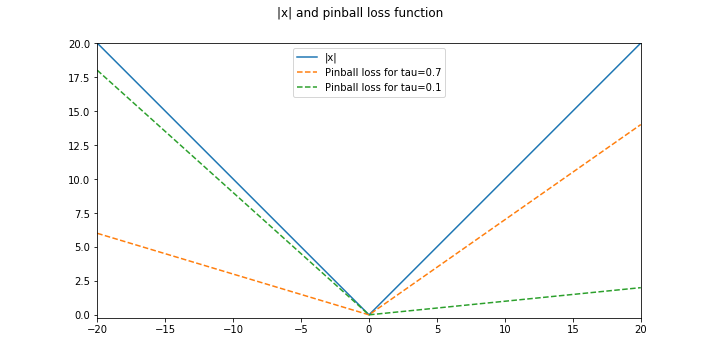
\includegraphics[width=1\columnwidth]{abs_pinball.png}
	\caption{Comparison between $|x|$ and the pinball loss function with different $\tau$ values}
\end{figure*}

The absolute function and the pinball loss function are obviously very much alike. In fact, with simple manipulation, the pinball loss function can be written in the form of absolute function as 
\begin{equation}
    l_\tau(x) = 
    \begin{cases}
        \tau \cdot |x| & {x \geq 0} \\
        (1-\tau) \cdot |x| & \text{otherwise}
    \end{cases}
\end{equation}
The pinball loss function is the combination of $|x|$ on the two parts $x<0$ and $x>0$ with different constant scale. 
If the derivative of the smooth function for $|x|$ at $x=0$ is $0$, we can also use the same approximation function respectively for the two parts of the pinball loss.
\\\\
In section \ref{subsec: smooth_sqrt} and \ref{subsec: smooth_new}, we show two approximation functions with regards to the absolute function $f = |x|$, along with the application of the approximations on the pinball loss function.

\subsection{Smooth function 1: a simple approximation}
\label{subsec: smooth_sqrt}

For $f = |x|$, a common and simple smooth approximation is $
    f = \sqrt{x^2 + \mu^2}
$.
 The convergence towards the absolute function is then proved by \citeauthor{voroninConvolutionBasedSmooth2015a}\cite{voroninConvolutionBasedSmooth2015a} that 
\begin{equation}
    ||x| - \sqrt{x^2 + \mu^2}| \leq \mu \text{  where } \mu > 0 \in \mathbb{R}
\end{equation}
\\
The smooth function application on the pinball loss function is:
\begin{equation}
    l_\tau(x) \approx 
    \begin{cases}
        \tau \cdot \sqrt{x^2 + \mu^2} & {x \geq 0} \\
        (1-\tau) \cdot \sqrt{x^2 + \mu^2} & {x < 0}
    \end{cases}
\end{equation}
and the derivative is
\begin{equation}
    l_\tau\prime(x) \approx 
    \begin{cases}
        \tau \cdot \frac{x}{\sqrt{x^2 + \mu^2}} & {x > 0} \\
        0 & {x=0} \\
        (1-\tau) \cdot \frac{x}{\sqrt{x^2 + \mu^2}} & {x<0}
    \end{cases}
\end{equation}
\subsection{Smooth function 2: a transcendental approximation}
\label{subsec: smooth_new}

For a better approximation accuracy, \citeauthor{bagulSMOOTHTRANSCENDENTALAPPROXIMATION2017}\cite{bagulSMOOTHTRANSCENDENTALAPPROXIMATION2017} proposes a new transcendental approximation function 
 \begin{equation}
    g(x) = x \cdot \tanh(x/\mu) \text{  where } \mu > 0 \in \mathbb{R}
 \end{equation}
which also satisfies
\begin{equation}
    ||x| - x \cdot tanh(\frac{x}{\mu})| < \mu
\end{equation}
The derivative of the approximation is
\begin{equation}
    \frac{dg(x)}{dx} = \frac{x}{\mu} \cdot sech^2 (\frac{x}{\mu}) + tanh(\frac{x}{\mu})
\end{equation}
For the pinball loss function, we now have its smooth function in the form:
\begin{equation}
    l_\tau(x) \approx 
    \begin{cases}
        \tau \cdot x \cdot \tanh(x/\mu) & {x\geq 0}\\
        (1-\tau) \cdot x \cdot \tanh(x/\mu) & {x < 0}
    \end{cases}
\end{equation}
and the derivative is
\begin{equation}
\label{eq:smooth_new_d}
    l_\tau\prime(x) \approx 
    \begin{cases}
        \tau \cdot \frac{x}{\mu} \cdot sech^2 (\frac{x}{\mu}) + tanh(\frac{x}{\mu}) & {x\geq 0}\\
        0 & {x=0}\\
        (1-\tau) \cdot \frac{x}{\mu} \cdot sech^2 (\frac{x}{\mu}) + tanh(\frac{x}{\mu}) & {x < 0}
    \end{cases}
\end{equation}
\subsection{Discussion and Conclusion}

In this part, we will compare the two alternative smooth functions in the following aspects: computer efficiency, approximation accuracy and
convexity. 
\begin{itemize}
    \item Computation efficiency: \\
    It is proved by \citeauthor{ramirezX2MostComputationally2014}\cite{ramirezX2MostComputationally2014} that $f = \sqrt{x^2 + \mu^2}$ is the most computationally efficient smooth approximation to $|x|$.
    
    On the other hand, we can see from equation \ref{eq:smooth_new_d}, the derivative for $g(x) = x · \tanh(x/\mu)$ is more difficult to compute.
    \item Approximation accuracy: \\
    The following plots show intuitively how fast the two smooth functions approach to $|x|$ for $\mu = 0.01$ and $\mu = 0.001$.
    
    \begin{figure*}[h!]
        \includegraphics[width=1\columnwidth]{{mu_0.001}.png}
        \caption{Comparison between the two smooth functions when $\mu = 0.001$}
    \end{figure*}

    \begin{figure*}[h!]
        \includegraphics[width=1\columnwidth]{{mu_0.0001}.png}
        \caption{Comparison between the two smooth functions when $\mu = 0.0001$}
    \end{figure*}

    We can see $ x \cdot \tanh(x/\mu)$ has a better accuracy.

    \item Convexity\\
    $f = \sqrt{x^2 + \mu^2}$ is convex and  $g(x) = x · \tanh(x/\mu)$ is not.
\end{itemize}

\textbf{Here we need a conclusion}
\textbf{Picure position is not forced to go with text position :(}



% \documentclass[11pt]{article}

\def\R{\rm I\!R}
\def\x{\bm{x}}
% \usepackage[margin=1in]{geometry}
% \usepackage{amssymb}
% \usepackage{amsmath}
% \usepackage{bm}
% \usepackage{xcolor}

\title{Stochastic Gradient Descent}

\begin{document}
\maketitle

\section{Stochastic Gradient Descent}

    Stochastic gradient descent (often abbreviated SGD) is an optimization algorithm developed from gradient descent. 
    In this section, gradient descent is introduced as the first part of the explanation of SGD.

    \subsection{Gradient Descent}
        For convex optimization problems, gradient descent is a first-order optimization algorithm 
        to find the local minimum of a function.
        \\\\
        To solve the minimization problem 
        $$ 
        \min_{\x} L(\x) 
        $$
        where $ L : \R^d \to \R$ is convex, differentiable and its gradient is Lipschitz continuous with constant
        $ L > 0$.
        \\\\
        Geometrically, the gradient $\nabla L(\x_0)$ points to the direction of the steepest ascent on $L(\cdot)$ 
        from the point $\x_0$. 
        By taking a small step in the direction of the negative gradient, the function value is decreased in the 
        direction of the steepest descent. That is,
        $$ 
        \x_1  = \x_0 - \alpha \nabla L(\x_0)
        $$
        for a small enough stepsize $\alpha \in \R_{+}$, then $L(\x_1) \leq L(\x_0)$. 
        That means, compared with $L(\x_0)$, $L(\x_1)$ is closer to the local minimum.
        \\\\
        With this observation comes the idea of gradient descent: an iterative "tour" on $L(\cdot)$ from a point towards the 
        local minimum by following small steps of negative gradient. 
        Let $\x_0$ be the guess of a starting point, then if
        $$
        \x_{k+1} = \x_{k} - \alpha_k \nabla L(\x_k), k \geq 0
        $$
        Then we have $ L(\x_0) \geq L(\x_1) \geq L(\x_2) \geq \cdots$ with suitable $\alpha_k$. The convergence of the 
        sequence $(\x_n)$ to the local minimum is guaranteed{\color{red} [reference]}.


    \subsection{Stochastic Gradient Descent}
        SGD can be considered as a stohcastic appoximation of gradient descent optimization, 
        when the objective function $L(\cdot)$ can be written as a sum of differentiable functions.
        Consider the objective function is in the form:
        $$
        L(\x) =\frac{1}{K} \sum_{k=1}^{K} L_k (\x)
        $$
        where the summand function $L_k$ is usually the loss function of the $k$th observation among
        $K$ data points.
        \\\\
        Then by following the idea of gradient descent, the $\x$ is updated according to
        $$
        \x_{k+1} = \x_{k} -\alpha_k \nabla L(\x_k) = \x_{k} -\alpha_k \frac{1}{K}\sum_{k=1}^{K} \nabla L_k(\x_k)
        $$
        where each $\alpha_k$ is a suitable stepsize. The calculation of $\sum_{k=1}^{K} \nabla L_k(\x_k)$ can be
        expensive, especially when the amount of summand functions is huge, or when the individual gradients are hard to
        compute. 
        \\\\
        To reduce the consumption of calculation, an estimation of the true gradient of $L(\x)$ is taken: 
        the true gradient $\frac{1}{K} \sum_{k=1}^{K} \nabla L_k(\x_k)$ is replaced by the gradient of a single observation $\nabla L_k(\x_k)$. 
        So the update of the parameter $\x$ becomes
        $$
        \x_{k+1} = \x_{k} - \alpha_k \nabla L_k(\x_k)        
        $$
        where $\alpha_k$ is a suitable stepsize. 
        \\\\
        The convergence of SGD has been proved as well{\color{red} [reference]}. 
        \\\\\\
        (and should I explain more about why stochastic gradient descent works?)


\end{document}
\end(documentclass)
% \documentclass[11pt]{article}

\def\R{\rm I\!R}
\def\x{\bm{x}}

\title{Proof of Algorithm Equivalence}
\author{Yiping Su}
\begin{document}
\maketitle
% --------------------------------------------------------------------------------
%                                Quantile Estimation
% --------------------------------------------------------------------------------
            
\section{Quantile Estimation}

\subsection{Quantile}

In statistics, quantiles are the points that divide a probability distribution into even intervals.
The $q$-quantiles devide the distribution into $q$ intervals each with the same amount of data points.
And there are $q$ quantile points of the $q-$quantiles.
For example, the $2$-quantile has only one quantile point, which is the middle point of the distribution
and it divides the distribution into two even parts. This $2$-quantile point is called the median.


\subsubsection{Definition} \label{tau-quantile-def}
Generally, the $q$-quantiles have $q-1$ quantile points, and the $k$th $q$-quantile for a 
distribution $X$ is the data value such that
$$
Pr(X \leq x) \geq \frac{k}{q}
$$
and
$$
Pr(X \geq x) \geq 1 - \frac{k}{q}
$$
where $x \in X$

\subsection{Quantile Estimation and Pinball Loss}
In this paper, the estimation for $\tau$-quantile 
($\tau =  \frac{1}{q}, \frac{2}{q}, \cdots, \frac{q-1}{q}$)
is applied.
Pinball loss function is one of the approaches for the estimation for a statistical population.
\\\\
For a one-dimentional data set $X = \{x_1, x_2, \cdots, x_N\}$, 
now consider the loss function for a single data point $x$ $(i \in {1, \cdots, N})$.
Let $t := x - q$ be the difference between the real value $x$ and the estimate of quantile $q$.
$l_{\tau}(\cdot): \R \to \R_{\geq 0}$ is the loss function on $t$ such that
$$
l_\tau(t)= 
    \begin{cases}
        \tau t & t > 0\\
        -(1-\tau) t & otherwise
    \end{cases}
$$
And the $\tau$-quantile loss has the {\color{red} subgradient}:
$$
\frac {\partial l_\tau(t)}{\partial t}= 
    \begin{cases}
        \tau                & t > 0\\
        -(1-\tau)           & t < 0\\
        [\tau, -(1 - \tau)] & t = 0
    \end{cases}
$$

The overall loss for distribution $X$ with quantile estimation $q$ is
$$
L_{\tau}(q) = \sum_{x \in X} l_{\tau}(x - q)
$$
The best estimate of the $\tau$-quantile $q$ is the $q$ with minimal overall loss. 
Let $q^\ast$ be the best estimate, then we have
$$
q^\ast = \argmin_{q} L_{\tau}(q)
$$


% --------------------------------------------------------------------------------
%                                SGD for Quantile Estimation
% --------------------------------------------------------------------------------
\section{Algorithm Equivalence}

\subsection{Pseudo Code for the Frugal-1U Algorithm}

Qiang Ma, S. Muthukrishnan and Mark Sandler {\color{red} [ref]}  
introduced the following algorithm \ref{alg:frugal_1U} which 
"uses only one unit of memory per group to compute a quantile for each group"({\color{blue} quotation}).

\begin{algorithm}
\caption{Frugal-1U}\label{alg:frugal_1U}
    \begin{algorithmic}[1]
        \Require{Data Stream $S$, $h$, $k$, $1$ unit of memory $\tilde{m}$}
        \Ensure{$\tilde{m}$}
        % \Procedure{frugal}{$X,\tau$}            \Comment{X is the dataset}
        \State {Initialization $\tilde{m} = 0$}               %\Comment{Default initialization $q_0$ = 0}
            \For{\textbf{each} $s_i$ in $S$}                  %\Comment{Parameter update for each input data point}
                \State{$rand$ = random(0,1); //get a random value in $[0,1]$}
                % \State {\textbf{set} $\alpha_k$} \Comment{Set stepsize}
                \If{$s_i > \tilde{m}$ \textbf{and} $rand > 1-\frac{h}{k}$} %\Comment{$q_{k+1} = q_k + \alpha_k \tau$ when $x_k - q_k > 0$}
                    \State{$\tilde{m} = \tilde{m} + 1$;}
                \Else { \textbf{if} $s_i < \tilde{m}$ \textbf{and} $rand > \frac{h}{k}$}  %\Comment{$q_{k+1} = q_k - \alpha_k (1-\tau)$ otherwise}
                    \State{$\tilde{m} = \tilde{m} - 1$;}
                \EndIf
            \State{\textbf{end if}}
            \EndFor
        \State{\textbf{end for}}
        % \State \textbf{return} $q$              \Comment{$q_k$ is the SGD result of quantile estimate}
        % \EndProcedure
    \end{algorithmic}
\end{algorithm}
The output $\tilde{m}$ is the estimate of the $h$th $k$-quantile for a given data stream $S$. 
By rephrasing of some steps of Frugal-1U, 
its equilalence to an SGD algorithm for quantile estimation will be shown in the follwing part.
\\\\
\textbf{Rephrasing of the Algorithm} \label{replacements}
\begin{enumerate}
    \item The constant $\frac{h}{k}$ is replaced by $\tau$, since the $\tau$-quantile is defined
     as the $h$th $k$-quantile point in section \ref{tau-quantile-def}.
    % \item The quantile estimate $\tilde{m}$ is replaced by $q$, as it stands for estimate of quantile.
    \item The generation of random number and it's comparison with $1-\frac{h}{k}$ or $\frac{h}{k}$
    in line 3 to 7 is replaced by the following algorithm.
    \begin{algorithm}
        \begin{algorithmic}[1]
            \setcounter{ALG@line}{2}
            \State{ }   \Comment{No need to generate a random number}
            \If{$s_i > \tilde{m}$} %\Comment{$q_{k+1} = q_k + \alpha_k \tau$ when $x_k - q_k > 0$}
                \State{$\tilde{m} = \tilde{m} + 1 \times (1-\frac{h}{k})$}     
                \Comment{$P((rand > 1-\frac{h}{k}) \mid rand \in \mathcal{U}(0,1)) = 1-\frac{h}{k}$;}
            \Else { \textbf{if} $s_i < \tilde{m}$}  %\Comment{$q_{k+1} = q_k - \alpha_k (1-\tau)$ otherwise}
                \State{$\tilde{m} = \tilde{m} - 1 \times \frac{h}{k}$}         
                \Comment{$P((rand > \frac{h}{k}) \mid rand \in \mathcal{U}(0,1)) = \frac{h}{k}$;}
            \EndIf 
        \end{algorithmic}
    \end{algorithm}

    % Here the probability $P((rand > p) \mid rand \in \mathcal{U}(0,1))$ is the simplification
    % for the generation of random number $rand$ and it's comparison to a constant $p$ $(0 < p < 1)$.
    
    To understand this replacement, let's consider the serie of the 3 steps: 
    (i) generate a random number $rand$, 
    (ii) compare it with a constant $p$, and
    (iii) take action if $rand > p$. 
    It can be interpreted as take the action with probability 
    $P((rand > p) \mid rand \in \mathcal{U}(0,1))$. 

    Mathmatically, the replacement works because the expected change of
    $\tilde{m}$ in both methods are the same. 
    For example when $s_i > \tilde{m}$, 
    the expected change of $\tilde{m}$ is
    $E_1[\nabla \tilde{m}] = E[\tilde{m} \times p]$ in the Frugal-1U with 
    random number generation,
    while 
    $E_2[\nabla \tilde{m}] = \tilde{m} \times p$ in the replacement method.
    Since $E_1[\nabla \tilde{m}] = E_2[\nabla \tilde{m}]$, the replacement is valid
    with regard to the expectation of the change in quantile estimate during each step.

\end{enumerate}


\subsection{SGD for Loss function}

Let $q_0$ be the initial guess of quantile estimate. 
By SGD, the estimate is updated each step with a data point from the distribution.
$$
q_{k+1} = q_k - \alpha_k g_k
$$
where $ \alpha_k $ is a suitable stepsize and 
$$
g_k = \partial L_{\tau}^{(k)}(q_k) \in \frac{\partial l_\tau(x_k - q_k)}{\partial q_k}
$$ 
\textbf{Notice: partial is taken because the gradient of a single variable function
euqals the partial of it}
\\\\
Then we have
$$
q_{k+1} = 
    \begin{cases}
        q_k + \alpha_k \tau               & x_k - q_k > 0\\
        q_k - \alpha_k (1-\tau)           & x_k - q_k \leq 0\\
        % [\tau, -(1 - \tau)] & t = 0
    \end{cases}
$$

\begin{algorithm}
    \caption{SGD algorithm}\label{alg:SGD}
    \begin{algorithmic}[1]
        \Require{Data Stream $X$, $\tau$, $1$ unit of memory $q$}
        \Ensure{$q$}
        % \Procedure{frugal}{$X,\tau$}            \Comment{X is the dataset}
        \State {Initialize} $q$                 \Comment{Default initialization $q_0$ = 0}
            \For{$x_k$ in $X$}                  \Comment{Parameter update for each input data point}
                \State \textbf{set} $\alpha_k$  \Comment{Set stepsize}
                \If{$x_k > q$}                  \Comment{$q_{k+1} = q_k + \alpha_k \tau$ when $x_k - q_k > 0$}
                    \State{$q = q + \alpha_k \tau$}
                \Else                           \Comment{$q_{k+1} = q_k - \alpha_k (1-\tau)$ otherwise}
                    \State{$q = q - \alpha_k (1-\tau)$}
                \EndIf
            \EndFor
        \State \textbf{return} $q$              \Comment{$q_k$ is the SGD result of quantile estimate}
        % \EndProcedure
    \end{algorithmic}
\end{algorithm}
% --------------------------------------------------------------------------------
%                              Equality of two algorithms 
% --------------------------------------------------------------------------------
\section{Equivalence of Algorithms}
In this section we'll show the equilalence of algorithm Frugal-1U 
and SGD.
\\\\
Besides the replacements mentioned in section \ref{replacements},
the notations have changed: 
$X$ is applied for the data stream, and $q$ instead of $\tilde{m}$
to represent quantile estimate.
The introduction of changable stepsize $\alpha_k$ for each data point $x_k$
is the highlight of the SGD algorithm. The flexibility of stepsize can help
with achieving a better convergence rate when stepsizes are chosen wisely.
Specifically, the setpsize is not mentioned in Frugal-1U 
because it is fixed as $1$. In SGD the stepsize might change for every step.

{\color{red} \textbf{Problem}}
In Frugal-1U the quantile estimate $q$ does not change when $x_k > q$, but in SGD 
the quantile estimate is updated: $q = q-\alpha_k (1-\tau)$. This can be seen as different 
\textbf{subgradient} values for $l_\tau(x_k - q_k)$ 
{\color{red} \textbf{but then I need to explain subgradient descent}} 


\end{document}


% \chapter{Simultaneously compute several quantiles in SGD}
\label{ch: simultaneous_quant}

Regression aims to find the relationship between dependent variables and independent variables. The parameters of the model is chosen by the methods for the regression (e.g. least squares).

In quantile regressions specifically wants to find the relation between quantile of $Y$ and the input $X$. The loss function chosen to tune the parameters is the pinball loss function: $\ell_{\tau}(r) = max(\tau r, (\tau - 1)r)$, where $r = y - q$ is the residual of $y$ minus the current quantile estimation. The function evaluates the performance of quantile estimation from a independent distribution $Y$. 

Quantile regression implements this function with the consideration that $Y$ is dependent on $X$, so the loss function looks like this:

\begin{equation}
    R_{\tau}^{\mathrm{emp}}(h)=\frac{1}{n} \sum_{i=1}^{n} \ell_{\tau}\left(y_{i}-h\left(\mathbf{x}_{i}\right)\right)
\end{equation}


where $h(\cdot)$ is the function for quantile estimator.

It is worth noticing that the quantile regression loss functions are generated from quantile estimation loss functions except for the dependence between variables. It means the loss functions applied in quantile regressions can be modified to implement in quantile estimation. Take the pinball loss function for example:
in quantile estimation, the dataset $X$ contains only one dimensional data points, and $Y$ is fully dependent on $X$. So the loss function to tune the estimation model is
\begin{equation}
    R_{\tau}^{\mathrm{emp}}(h)=\frac{1}{n} \sum_{i=1}^{n} \ell_{\tau}\left(y_{i}-h\left(\mathbf{x}_{i}\right)\right)
        = \frac{1}{n} \sum_{i=1}^{n} \ell_{\tau}\left(x_{i}-h\left({x}_{i}\right)\right) 
        = \frac{1}{n} \sum_{i=1}^{n} \ell_{\tau}\left(x_{i}- q^{est}\right) 
\end{equation}

in which the quantile estimator $h\left(\mathbf{x}_{i}\right)$ is replaced with the constant quantile estimate $q^{est}$.

In the quantile regression method, there is another loss function aims to reduce the crossing between different quantile values:

\begin{equation}
    \sum_{j=1}^{p-1}\left[\frac{1}{n} \sum_{i=1}^{n} \max \left(0, h_{j+1}\left(\mathbf{x}_{i}\right)-h_{j}\left(\mathbf{x}_{i}\right)\right)\right]
\end{equation}


Where $p$ is the total amount of $\tau$ values that needs to be estimated simultaneously, and here we assume$(\tau_j > \tau_{j+1})$.


To apply it in quantile estimation, the dependence between $Y$ and $X$ should be reduced from the loss function. Luckily the relationship is not included at all in the regression loss function. So for quantile estimation we can use
\begin{equation}
    \sum_{j=1}^{p-1}\left[\frac{1}{n} \sum_{i=1}^{n} \max \left(0, h_{j+1}\left({x}_{i}\right)-h_{j}\left({x}_{i}\right)\right)\right]
= \sum_{j=1}^{p-1}\left[\frac{1}{n} \sum_{i=1}^{n} \max \left(0, q_{j+1}^{est}-q_{j}^{est}\right)\right]
\end{equation}



% \documentclass[12pt]{article}
\usepackage{xcolor}
\usepackage[nointegrals]{wasysym}

\def\R{\rm I\!R}
\def\x{\bm{x}}

\title{SGD Quantile Estimation Experiement}
\date{\vspace{-5ex}}

\begin{document}
\maketitle

\section{Introduction}

% \subsection你说“我就不该这么想”{Aims}
This experiment has two purposes. The first is to show quantile estimation with SGD works \textcolor{blue}{ under some circimstances (?)}.
The second aim is to investigate how different settings of the problem effect the estimation performance. Specifically, we are interested in the following aspects: data distribution, data size, data ordering, quantile value and sgd step size.
In the experiment, multiple ordered datasets are generated as input data streams, based on which the calculated and estimated quantile values are computed. Results of both quantiles are compared after processing. We want to compare the performance of quantile estimation over different settings.
\\\\
\textcolor{blue}{This experiment also aims at the comparison between Frugal algorithm and SGD algorithm, by which we want to show that those two algorithms are ``equivalent". 
\\
(Does it mean SGD estimation works?)}
% To test the SGD quantile estimation as a valid alternative for quantile estimation, this experiment computes both estimated and calculated values for quantiles, and evaluates whether the difference between the results is acceptable.
% \\\\
% Do I explain the second goal...?


\section{Methodology}
The process by which we experiment on SGD quantile estimation can be briefly outlined as followes:

\begin{enumerate}
    \item Select a set of data streams (ordered datasets) derived from some statistical distributions.
    \item For each $\tau$-quantile, determine a ground truth value from the distribution and calculate a empirical value from the data stream.
    \item For each $\tau$-quantile, calculate the SGD estimate value from the data stream, record both the process and the result of estimation.
    \item \textcolor{blue}{
        Compare Frugal algorithm and SGD algorithm on data streams of the same setting.
    }
    \item Compute normalized error value for quantile estimates as a measurement of similarity between empirical and estimate value. The error value is computed from both values.
\end{enumerate}

\subsection{Data Stream Set Generation}
A total of 4 distributions are used in this experiment.
Eah data stream is a set of 1 dimensional data points randomly sampled from one of the distributions. In order to show how the amount of data points might affect the performance, there are 3 different settings for the data size $N$. 
\\\\
Each data stream set is composed of a number of data streams. For a statistically more accurate results on the experiment, a group of data streams of the same settings are generated. When investigating the impact of data sequence has on quantile estimation, one data stream will be shuffled to for the generation to differently ordered data steams. To sum up, a data stream set is either a combination of data streams generated from same distribution and data size setting, or the permutations of one same data stream. We generate the data stream set under this settings:

\begin{itemize}
    \item Distribution: 4 statistical distributions. The 4 distributions are:
        \begin{itemize}
            \item Gaussian distribution 1: mean = 2, standard deviation = 18
            \item Gaussian distribution 2: mean = 0, standard deviation = 0.001
            \item Exponetial distribution: rate = 1
            \item Mixed Gaussian distribution: a mix of five different gaussian distributions
        \end{itemize}
    \item Data size: 100, 1000, 10000, 100000(?)
    \item Multiple generations: True or false. Generate 10 data streams for the set if true.
    \item Multiple shuffles:  True or false. Shuffle the data stream 10 times for the set if true.
\end{itemize}

\subsection{True and Empirical Quantile Calculation}
The true quantile values are the quantile values for the distributions which the data streams are derived from. They are calculated by the maths functions for quantile computation. All except the mixed gaussian distribution has a relatively easy function for quantile calculation. For the mixed distribution, the empirical quantile value from a large amount of sampling is taken for the true value. By this means, the empirical value is expected to be close enough to the true quantile value such that the evaluation of results is not much affected \textcolor{blue}{(needs more justification?)}. In this experiment, a total of 100,000,000 samples are generated for the calculation. For a certain $\tau$, there is only one true quantile value for one distribution.
\\\\
The empirical quantile value is the quantile value calculated from the data steam instead of the distribution. For a certain $\tau$, no matter what the ordering is, there is only one empirical quantile value for one data stream, but there can be multiple quantile values for one distribution.

\subsection{SGD Quantile Estimation}

The parameter of SGD quantile estimation is important. The current settings for step size $\alpha_k$ are:
\begin{itemize}
    \item Constant number: $\alpha_k =1$
    \item Decrease when k increases: $\alpha_k = \frac{2}{\sqrt{k}}$
    \item Decrease when k increases (smaller size): $\alpha_k = \frac{0.002}{\sqrt{k}}$
\end{itemize}
where $k$ is the index of step count.
\subsection{Frugal and SGD algorithm}

Frugal algorithm is proposed for quantile estimation as well. In this experiment, we want to compare the two algorithms and show they have similar performance for same data streams. In this experiment, data streams are generated from all 4 distributions, and the step size for SGD quantile estimation is set to constant 1.

\subsection{Error Computation}

An error measurement is proposed in order to evaluate the performance of quantile estimation. The error value represents the difference between empirical and estimated quantile value. For one data stream, the error function for its $\tau$-quantile is first defined as $E^{(\tau)} = | q_{batch}^{(\tau)} - q_{sgd}^{(\tau)} |$, where $E^{(\tau)}$ stands for the error, $q_{batch}^{(\tau)}$ for empirical quantile value and $q_{sgd}^{(\tau)}$ for SGD estimate value. For a specific data stream, a smaller $E^{(\tau)}$ means the estimation for the $\tau$-quantile has a better accuracy. Generally, for $n$ data streams of same size and distribution, we take the mean of the error value $\overline{E^{(\tau)}}$, where 
    $$
        \overline{E^{(\tau)}} = \frac{1}{n}\sum_{i=1}^{n} E^{(\tau)}_{i}
    $$
where $E^{(\tau)}_{i}$ is the error value of $\tau$-quantile for the $i$th data stream. To compare the performance of different settings of SGD estimation, we can now compare the $\overline{E^{(\tau)}}$ value for each setting.
\\\\
 Despite the capability of accuracy comparison, there is still room for improvement for this preliminary error measurement. 
% distribution
 First, the limitation of data distribution. The comparison is only available for data streams generated from the same distribution, since a different distribution has difference density of data points for the same $\tau$ value, leading to a failure of error comparison. For example, a data stream generated from uniform distribution $\mathcal{U}(0,1)$, the error value $\overline{E^{(0.1)}} = 2$ is a bad estimation, because 2 is even greater than the difference between the minimal and maximal value of the distribution ($2 > |0-1|$). However, for a data stream sampled from uniform distribution $\mathcal{U}(0,10^{10})$, $\overline{E^{(0.1)}} = 2$ might be a really accurate result, given how low the density is around its 0.1-quantile. 
% tau
 Second, the limitation of $\tau$ value. Similarly with the distribution problem, different $\tau$ values in the same distribution may have varied density. For example, for a gaussian distribution, $\overline{E^{(0.01)}} = \overline{E^{(0.5)}}$ means that the estimation is better for 0.01-quantile than 0.5-quantile, since the distribution is denser around the middle than its outlier.
% how it works
 Third and more importantly, it is incapable of showing if the estimation "works". Specifically, for some number $x$, we cannot find a reasonable explanation for the statement ``the estimate is accurate enough because we have $\overline{E^{(\tau)}} \leq x$''. Since for any $x$, we could find an example from the first two issues as a counter example. To solve those problems, a more general comparison of accuracy should be enabled by the new error measurement.
\\\\
In the new version of error value calculation, true quantile value of a data distribution $q_{true}^{(\tau)}$ is involved, so that $E^{(\tau)}$ is normalized by $|q_{batch}^{(\tau)} - q_{true}^{(\tau)}|$. It is now defined as
$$
    E^{(\tau)} = \frac{|q_{batch}^{(\tau)} - q_{sgd}^{(\tau)}|}
                      {|q_{batch}^{(\tau)} - q_{true}^{(\tau)}|}
$$
So that the accuracy of $q_{sgd}^{(\tau)}$ is compared with the accuracy of $q_{batch}^{(\tau)}$. The above problem is solved because \textcolor{orange}{to be continued}

\section{Observations}


\section{Discussion? Accuracy of study?}
% \begin{equation}
%     E = | \frac{q_{batch} - q_{sgd}}{{q_{batch}}^{(1)} - {q_{batch}}^{(2)}} |
% \end{equation}
\section{Conclusion}

\end{document}
\end(documentclass)

\cleardoublepage % Empty page before the start of the next part

%------------------------------------------------
% part 2

% \ctparttext{You can put some informational part preamble text here. Illo principalmente su nos. Non message \emph{occidental} angloromanic da. Debitas effortio simplificate sia se, auxiliar summarios da que, se avantiate publicationes via. Pan in terra summarios, capital interlingua se que. Al via multo esser specimen, campo responder que da. Le usate medical addresses pro, europa origine sanctificate nos se.} % Text on the Part 2 page describing the content in Part 2

% \cleardoublepage % Empty page before the start of the next part
% \appendix
% \part{Appendix} % New part of the thesis for the appendix

%----------------------------------------------------------------------------------------
%	THESIS CONTENT - APPENDICES
%----------------------------------------------------------------------------------------

% \include{Chapters/Chapter0A} % Appendix A
%\include{Chapters/Chapter0B} % Appendix B - empty template

%----------------------------------------------------------------------------------------
%	POST-CONTENT THESIS PAGES
%----------------------------------------------------------------------------------------

\cleardoublepage% Bibliography

\label{app:bibliography} % Reference the bibliography elsewhere with \autoref{app:bibliography}

\manualmark % Work-around to have small caps also here in the headline
\markboth{\spacedlowsmallcaps{\bibname}}{\spacedlowsmallcaps{\bibname}} % Work-around to have small caps also
%\phantomsection
\refstepcounter{dummy}

\addtocontents{toc}{\protect\vspace{\beforebibskip}} % Place the bibliography slightly below the rest of the document content in the table of contents
\addcontentsline{toc}{chapter}{\tocEntry{\bibname}}

\printbibliography % Bibliography

% \cleardoublepage% Declaration

\refstepcounter{dummy}
\pdfbookmark[0]{Declaration}{declaration} % Bookmark name visible in a PDF viewer

\chapter*{Declaration} % Declaration section text

\thispagestyle{empty}

Put your declaration here.
\bigskip
 
\noindent\textit{\myLocation, \myTime}

\smallskip

\begin{flushright}
\begin{tabular}{m{5cm}}
\\ \hline
\centering\myName \\
\end{tabular}
\end{flushright}
 % Declaration


%----------------------------------------------------------------------------------------

\end{document}
